\section{三角恒等变换}
\subsection{两角和、差的三角函数}
    \ref{subsec_诱导公式}节诱导公式说明了$\alpha$与$\pm \alpha \pm \frac{n\pi}{2}$的三角函数关系。
    ，但如果\(\frac{\pi}{2}\)变为一个特殊的角呢？对于一般的情况，是否有
    \[\cos(\alpha+\beta) = \cos \alpha+cos \beta\]
    这样美好的公式呢？带入几个特殊的角，发现这是不可能的……下面这个定理给出真正的两角和的余弦公式。
\begin{theorem}[两角和的余弦]\label{两角和余弦定理}
    $\forall \alpha,\beta \in \mathbb{R} $满足
    \begin{equation}
        \cos(\alpha+\beta) = \cos \alpha\cos \beta -\sin \alpha\cos \beta  
    \end{equation}
\end{theorem}
\begin{proof}
    先考虑$\alpha,\beta$都是锐角的情况。在单位圆中画出$\aa$，$\bb$和$-\bb$。
    \begin{figure}[htbp]
    \centering
    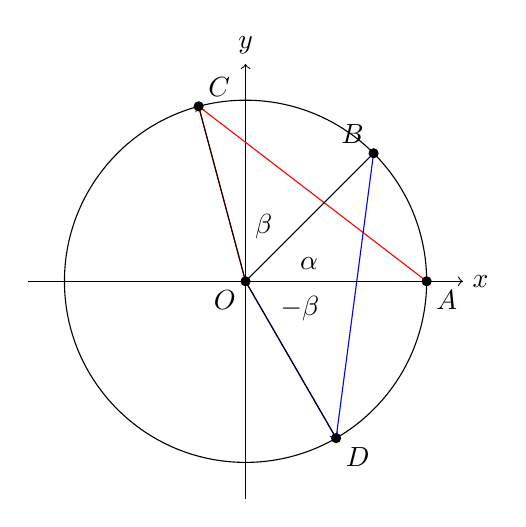
\begin{tikzpicture}[scale=2.3]
      \coordinate (O) at (0,0);
      \draw[->] (-1.2,0) -- (1.2,0) node[right] {$x$};
      \draw[->] (0,-1.2) -- (0,1.2) node[above] {$y$};
      \draw (0,0) circle [radius=1];
      \coordinate (A) at (1,0);
      \coordinate (B) at (0.707,0.707);
      \coordinate (C) at (-0.259,0.966);
      \coordinate (D) at (0.5,-0.866);
      \draw[->,red] (O) -- (C);
      \draw[->,blue] (O) -- (D);
      \draw[red] (A) -- (C);
      \draw[blue] (B) -- (D);
      \draw (O) -- (A) node[midway,below] {};
      \draw (O) -- (B) node[midway,left] {};
      \draw (O) -- (C) node[midway,above left] {};
      \draw (O) -- (D) node[midway,below left] {};
      \fill (O) circle (0.8pt) node[below left] {$O$};
      \fill (A) circle (0.8pt) node[below right] {$A$};
      \fill (B) circle (0.8pt) node[above left] {$B$};
      \fill (C) circle (0.8pt) node[above right] {$C$};
      \fill (D) circle (0.8pt) node[below right] {$D$};
      \node at (0.35,0.1) {$\alpha$};
      \node at (0.1,0.3) {$\beta$};
      \node at (0.3,-0.15) {$-\beta$};
    \end{tikzpicture}
    \end{figure}

    其中$A(1,0)$，$B(\cos\aa,\sin\aa)$，$C(\cos(\aa+\bb),\sin(\aa+\bb))$，$D(\cos(-\bb),\sin(-\bb))=(\cos\bb,-\sin\bb)$。
    由于圆的半径相等，$\angle AOC=\angle BOD=\aa+\bb$，故$\triangle AOC\cong \triangle BOD(SAS)$，
    因此有$|AC|=|BD|$。
    
    即
    \begin{align*}
        (\cos^2(\aa+\bb)-1)^2+\sin^2(\aa+\bb)&=(\cos\aa-\cos\bb)^2+(\sin\aa+\sin\bb)^2\\
        \cos^2(\aa+\bb)-2\cos(\aa+\bb)+1+\sin^2(\aa+\bb)&=\cos^2\aa-2\cos\aa\cos\bb+\cos^2\bb+\sin^2\aa+2\sin\aa\sin\bb+\sin^2\bb\\
        1-2\cos(\aa+\bb)+1&=1+1-2\cos\aa\cos\bb+2\sin\aa\sin\bb\\
        \cos(\alpha+\beta)& = \cos \alpha\cos \beta -\sin \alpha\cos \beta  
    \end{align*}

    在这里用到了之前证明过的$\sin^2\aa+\cos^2\bb=1\quad(\forall\aa\in\mathbb{R})$.
\end{proof}

接下来就可以利用定理\ref{两角和余弦定理}来证明接下来的五个式子
\begin{theorem}
    $\forall \alpha,\beta \in \mathbb{R} $满足
    \begin{equation}\label{两角差余弦}
        \cos(\alpha-\beta) = \cos \alpha\cos \beta +\sin \alpha\cos \beta  
    \end{equation}
    \begin{equation}\label{两角和正弦}
        \sin(\aa+\bb)=\sin\aa\cos\bb+\cos\aa\sin\bb
    \end{equation}
    \begin{equation}\label{两角差正弦}
        \sin(\aa-\bb)=\sin\aa\cos\bb-\cos\aa\sin\bb
    \end{equation}
    \begin{equation}\label{两角和正切}
        \tan(\aa+\bb)=\frac{\tan\aa+\tan\bb}{1-\tan\aa\tan\bb}
    \end{equation}
    \begin{equation}\label{两角差正切}
        \tan(\aa-\bb)=\frac{\tan\aa-\tan\bb}{1+\tan\aa\tan\bb}
    \end{equation}
\end{theorem}
\begin{proof}
仅证明
\end{proof}

\begin{theorem}[正弦平方差]
    \begin{equation}
         \sin^2\alpha - \sin^2\beta = \sin(\alpha+\beta)\sin(\alpha-\beta) 
    \end{equation}
\end{theorem}
\begin{proof}
    利用正弦函数的和角与差角公式：
\[
\begin{aligned}
\sin(\alpha+\beta) &= \sin\alpha\cos\beta + \cos\alpha\sin\beta \\
\sin(\alpha-\beta) &= \sin\alpha\cos\beta - \cos\alpha\sin\beta
\end{aligned}
\]
将两式相乘：
\[
\begin{aligned}
\mathrm{RHS} &= (\sin\alpha\cos\beta + \cos\alpha\sin\beta)(\sin\alpha\cos\beta - \cos\alpha\sin\beta) \\
&= (\sin\alpha\cos\beta)^2 - (\cos\alpha\sin\beta)^2 \\
&= \sin^2\alpha\cos^2\beta - \cos^2\alpha\sin^2\beta\\
&= \sin^2\alpha(1-\sin^2\beta) - (1-\sin^2\alpha)\sin^2\beta \\
&= \sin^2\alpha - \sin^2\alpha\sin^2\beta - \sin^2\beta + \sin^2\alpha\sin^2\beta \\
&= \sin^2\alpha - \sin^2\beta =\mathrm{LHS}
\end{aligned}
\]
其中利用了恒等式 $\cos^2 x = 1 - \sin^2 x$.
\qed
\end{proof}


\begin{corollary}
     \begin{align*}
    \cos^2\alpha - \cos^2\beta &= -\sin(\alpha+\beta)\sin(\alpha-\beta) \\
    \cos^2\alpha - \sin^2\beta &= \cos(\alpha+\beta)\cos(\alpha-\beta) \\
    \sin^2\alpha - \cos^2\beta &= -\cos(\alpha+\beta)\cos(\alpha-\beta)
\end{align*}
\end{corollary}
\begin{proof}
    \qed
\end{proof}


















\clearpage
\subsection{二倍角公式及其拓展}
\clearpage
\subsection{积化和差与和差化积}
\begin{theorem}
    \begin{equation}
        \sin\alpha \sin\beta = \frac{1}{2}[\cos(\alpha - \beta) - \cos(\alpha + \beta)]
    \end{equation}
        
    \begin{equation}
        \cos\alpha \cos\beta = \frac{1}{2}[\cos(\alpha - \beta) + \cos(\alpha + \beta)]
    \end{equation}
        
    \begin{equation}
        \sin\alpha \cos\beta = \frac{1}{2}[\sin(\alpha + \beta) + \sin(\alpha - \beta)]
    \end{equation}
        
    \begin{equation}
        \cos\alpha \sin\beta =\frac{1}{2} [\sin(\alpha + \beta) - \sin(\alpha - \beta)]
    \end{equation}
\end{theorem}
\begin{theorem}
    

    \begin{equation}
        \sin\alpha + \sin\beta = 2 \sin\left(\frac{\alpha + \beta}{2}\right) \cos\left(\frac{\alpha - \beta}{2}\right)
    \end{equation}
        
    \begin{equation}
        \sin\alpha - \sin\beta = 2 \cos\left(\frac{\alpha + \beta}{2}\right) \sin\left(\frac{\alpha - \beta}{2}\right)
    \end{equation}
        
    \begin{equation}
        \cos\alpha + \cos\beta = 2 \cos\left(\frac{\alpha + \beta}{2}\right) \cos\left(\frac{\alpha - \beta}{2}\right)
    \end{equation}
        
    \begin{equation}
        \cos\alpha - \cos\beta = -2 \sin\left(\frac{\alpha + \beta}{2}\right) \sin\left(\frac{\alpha - \beta}{2}\right)
    \end{equation}
\end{theorem}

\begin{example}
    求满足下列条件的区域的面积：
    \[\{(x,y)|x,y\in[0,\frac{\pi }{2}],\sin ^2 x-\sin x \sin y+\sin ^2y\leq\frac{3}{4}\}\]
\end{example}

\begin{jie}
\begin{way1}
    对不等式左侧的式子做变换
\begin{align}
     &\sin ^2 x-\sin x \sin y+\sin ^2y \notag\\ 
     =&\frac{1}{2}(1-\cos 2x-(\cos(x-y)-\cos(x+y))+1-\cos2y)\label{积化和差求面积1}\\
     =&\frac{1}{2}(2-2\cos(x+y)\cos(x-y)-\cos(x-y)+\cos(x+y))\label{积化和差求面积2}
\end{align}
   式\ref{积化和差求面积1}是对\(\sin x\sin y\)作积化和差得到的的
   ，式\ref{积化和差求面积2}是对\(\cos 2x+\cos 2y\)作和差化积得到的。
   
   故原不等式可以变为
   \[2\cos(x+y)\cos(x-y)+\cos(x-y)-\cos(x+y)-\frac{1}{2}\geq 0\]
   因式分解得
   \[(2\cos(x+y)+1)(\cos(x-y)-\frac{1}{2})\geq 0\]
   解得
 \begin{equation}\label{积化和差求面积3}
      \left\{\begin{array} { l } 
       \displaystyle{ \cos(x + y) \leqslant -\frac { 1 } { 2 }  } \\
       \displaystyle{ \cos(x - y) \leqslant \frac{1}{2}}
       \end{array} \text { 或 } \left\{\begin{array}{l}
       \displaystyle\cos(x + y) \geqslant -\frac { 1 } { 2 } \\
       \displaystyle\cos(x - y) \geqslant \frac{1}{2}
       \end{array}\right.\right.
 \end{equation}

    由于\(x,y\in[0,\dfrac{\pi }{2}]\)，故可以确定
    \[0\leq x+y\leq\pi,-\frac{\pi}{2}\leq x-y\leq \frac{\pi}{2}\]

    结合不等式组\ref{积化和差求面积3}，列出下面的不等式组
   \[\left\{\begin{array} { l } 
    \displaystyle{0 \leq x + y \leqslant \frac { 2 } { 3 }\pi  } \\
    \displaystyle{-\frac{\pi}{3} \leq x - y \leq \frac { \pi } { 3 } }
    \end{array} \text { 或 } \left\{\begin{array}{l}
    \displaystyle \frac{2 }{3}\pi\leq x+y \leq \pi \\
    \displaystyle\frac{\pi}{3}\leq x-y  \leq \frac{\pi}{2} \text{或}-\frac{\pi}{2}\leq x-y  \leq -\frac{\pi}{3}
    \end{array}\right.\right.\]

    如下图所示在平面直角坐标系中绘制出两个不等式组对应的区域：
    %\sout{思考：请利用此题计算}\[{\sum_{n=1}^{+\infty}\frac{1}{n^2}}\]

    \begin{figure}[h]
        \centering
        
        \begin{subfigure}[h]{0.45\textwidth}
            \centering
            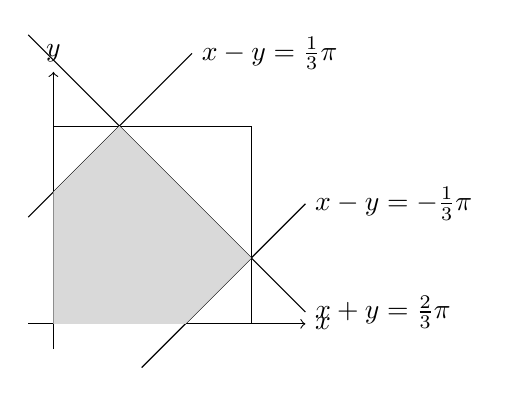
\begin{tikzpicture}[
                scale=1.6, % 调整比例
            ]
            % 定义坐标轴
            \draw[->] (-0.2,0) -- (2,0) node[right] {$x$};
            \draw[->] (0,-0.2) -- (0,2) node[above] {$y$};
            \draw (0,0) rectangle (1.57,1.57);
            % 定义直线的坐标
            \def\lineA{(-0.2, {2/3*3.14159 +0.2}) -- (2, {2/3*3.14159 -2})}
            \def\lineB{(-0.2, {1/3*3.14159 -0.2}) -- (1.1, {1/3*3.14159 + 1.1})}
            \def\lineC{(0.7, {-1/3*3.14159+0.7}) -- (2, {-1/3*3.14159 + 2})}
            
            % 画直线
            \draw \lineA node[right] {$x+y=\frac{2}{3}\pi$};
            \draw \lineB node[right] {$x-y=\frac{1}{3}\pi$};
            \draw \lineC node[right] {$x-y=-\frac{1}{3}\pi$};
            
            % 填充灰色区域
            \coordinate (A) at (0,0);
            \coordinate (B) at (0,{pi/3});
            \coordinate (C) at ({pi/6},{pi/2});
            \coordinate (D) at ({pi/2},{pi/6});
            \coordinate (E) at ({pi/3},0); % 闭合路径
            \fill[gray!30] (A) -- (B) -- (C) -- (D) -- (E)--cycle;
            \end{tikzpicture}
            \caption{情况1}
        \end{subfigure}%
        \hfill
        \begin{subfigure}[h]{0.45\textwidth}
            \centering
            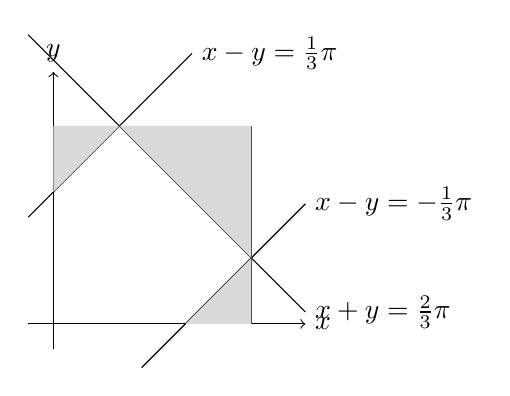
\begin{tikzpicture}[
                scale=1.6, % 调整比例
            ]
            % 定义坐标轴
            \draw[->] (-0.2,0) -- (2,0) node[right] {$x$};
            \draw[->] (0,-0.2) -- (0,2) node[above] {$y$};
            \draw (0,0) rectangle (1.57,1.57);
            % 定义直线的坐标
            \def\lineA{(-0.2, {2/3*3.14159 +0.2}) -- (2, {2/3*3.14159 -2})}
            \def\lineB{(-0.2, {1/3*3.14159 -0.2}) -- (1.1, {1/3*3.14159 + 1.1})}
            \def\lineC{(0.7, {-1/3*3.14159+0.7}) -- (2, {-1/3*3.14159 + 2})}
            
            % 画直线
            \draw \lineA node[right] {$x+y=\frac{2}{3}\pi$};
            \draw \lineB node[right] {$x-y=\frac{1}{3}\pi$};
            \draw \lineC node[right] {$x-y=-\frac{1}{3}\pi$};
            
            % 填充灰色区域
            \coordinate (A) at (0,0);
            \coordinate (B) at (0,{pi/3});
            \coordinate (C) at ({pi/6},{pi/2});
            \coordinate (D) at ({pi/2},{pi/6});
            \coordinate (E) at ({pi/3},0);
            \coordinate (F) at (0,{pi/2}); % 闭合路径
            \coordinate (G) at ({pi/2},{pi/2});
            \coordinate (H) at ({pi/2},0);
            \fill[gray!30] (B) -- (F) -- (C)--cycle;
            \fill[gray!30] (C) -- (G) -- (D)--cycle;
            \fill[gray!30] (D) -- (H) -- (E)--cycle;
            \end{tikzpicture}
            \caption{情况2}
        \end{subfigure}
        \caption{由上不等式组绘制出的图像}
        \label{积化和差求面积图像}
    \end{figure}

    上图中情况1对应着左侧的不等式组，灰色阴影部分为各个不等式的交集，即为题目所求区域
    ；情况2对应着右侧的不等式组，最后要求取三个灰色部分的交集，这是不可能的，故无解。

 综上所述，最终原题目中的面积为正方形面积减去三个三角形面积：
    \[S=\left(\frac{\pi}{2}\right)^2-2\times\frac{1}{2}\left(\frac{\pi}{6}\right)^2-\frac{1}{2}\left(\frac{\pi}{3}\right)^2=\frac{\pi^2}{6}\]
\end{way1}

\begin{way2}
    仅仅考虑边缘部分，
    \begin{equation}
        \sin^2 x-\sin x\sin y+\sin^2 y=\frac{3}{4}
    \end{equation}
    对其配方\footnote{这个操作不太习惯也没关系，在二次型可以学习到类似的技巧。}，得到
    \begin{equation}
        \frac{1}{3}(\sin x +\sin y)^2+(\sin y-\sin x)^2=1
    \end{equation}
    不妨设
    \[
   \left\{
        \begin{array} { l } 
        \sin x+\sin y=\sqrt{3} \sin t\\
        \sin y-\sin x=\cos t
        \end{array}
    \right.
    \]
    解得
        \[
   \left\{
        \begin{array} { l } 
        \displaystyle \sin x=\frac{1}{2}(\sqrt{3} \sin t-\cos t)=\sin(t-\frac{\pi}{6})\\
        \displaystyle \sin y=\frac{1}{2}(\sqrt{3} \sin t+\cos t)=\sin(t+\frac{\pi}{6})
        \end{array}
    \right.
    \]

    利用正弦函数的性质脱掉\(\sin\)的外壳得到：
    \begin{equation}\label{积化和差求面积方程1}
        x=t-\frac{\pi}{6}+2k\pi\ (k\in \mathbb{Z})
    \end{equation}
    \begin{equation}\label{积化和差求面积方程2}
        x+t-\frac{\pi}{6}=\pi+2k\pi\ (k\in \mathbb{Z})
    \end{equation}
    \begin{equation}\label{积化和差求面积方程3}
        y=t+\frac{\pi}{6}+2k\pi\ (k\in \mathbb{Z})
    \end{equation}
    \begin{equation}\label{积化和差求面积方程4}
        y+t+\frac{\pi}{6}=\pi+2k\pi\ (k\in \mathbb{Z})
    \end{equation}
    两两消去参数\(t\)得到三组平行直线系方程：
    \begin{equation}
        y-x=\frac{\pi}{3}+2k\pi  \ (\ref{积化和差求面积方程3}-\ref{积化和差求面积方程1},k\in \mathbb{Z})
    \end{equation}
    \begin{equation}
        x+y=\frac{2}{3}\pi+2k\pi \ (\ref{积化和差求面积方程1}+\ref{积化和差求面积方程4}\text{或}\ref{积化和差求面积方程2}+\ref{积化和差求面积方程3},k\in \mathbb{Z})
    \end{equation}
    \begin{equation}
        x-y=\frac{\pi}{3}+2k\pi\ (\ref{积化和差求面积方程2}-\ref{积化和差求面积方程4},k\in \mathbb{Z})
    \end{equation}


    结合\(x,y\in[0,\dfrac{\pi}{2}]\)，即可确定是
    \[x-y+\frac{\pi}{3}=0\]
    \[x-y-\frac{\pi}{3}=0\]
    \[x+y-\frac{2}{3}\pi=0\]仍然可以绘制出图\ref{积化和差求面积图像}，但是这仅仅确定了边界，具体是哪块区域
    可以通过代入特殊点来确定。
\end{way2}

\begin{way3}
同法2一样，仍然先考虑边界。注意到原式的形式类似余弦定理
\end{way3}



\end{jie}




\clearpage
\subsection{三角函数的其他定义*}
\clearpage
\subsection{反三角函数的恒等变换**}
\clearpage
\review
\clearpage
\hw
\clearpage
